\documentclass[tikz,border=10pt]{standalone}
\usepackage{tikz}
\usetikzlibrary{shapes,arrows,positioning,fit,shadows}

\begin{document}
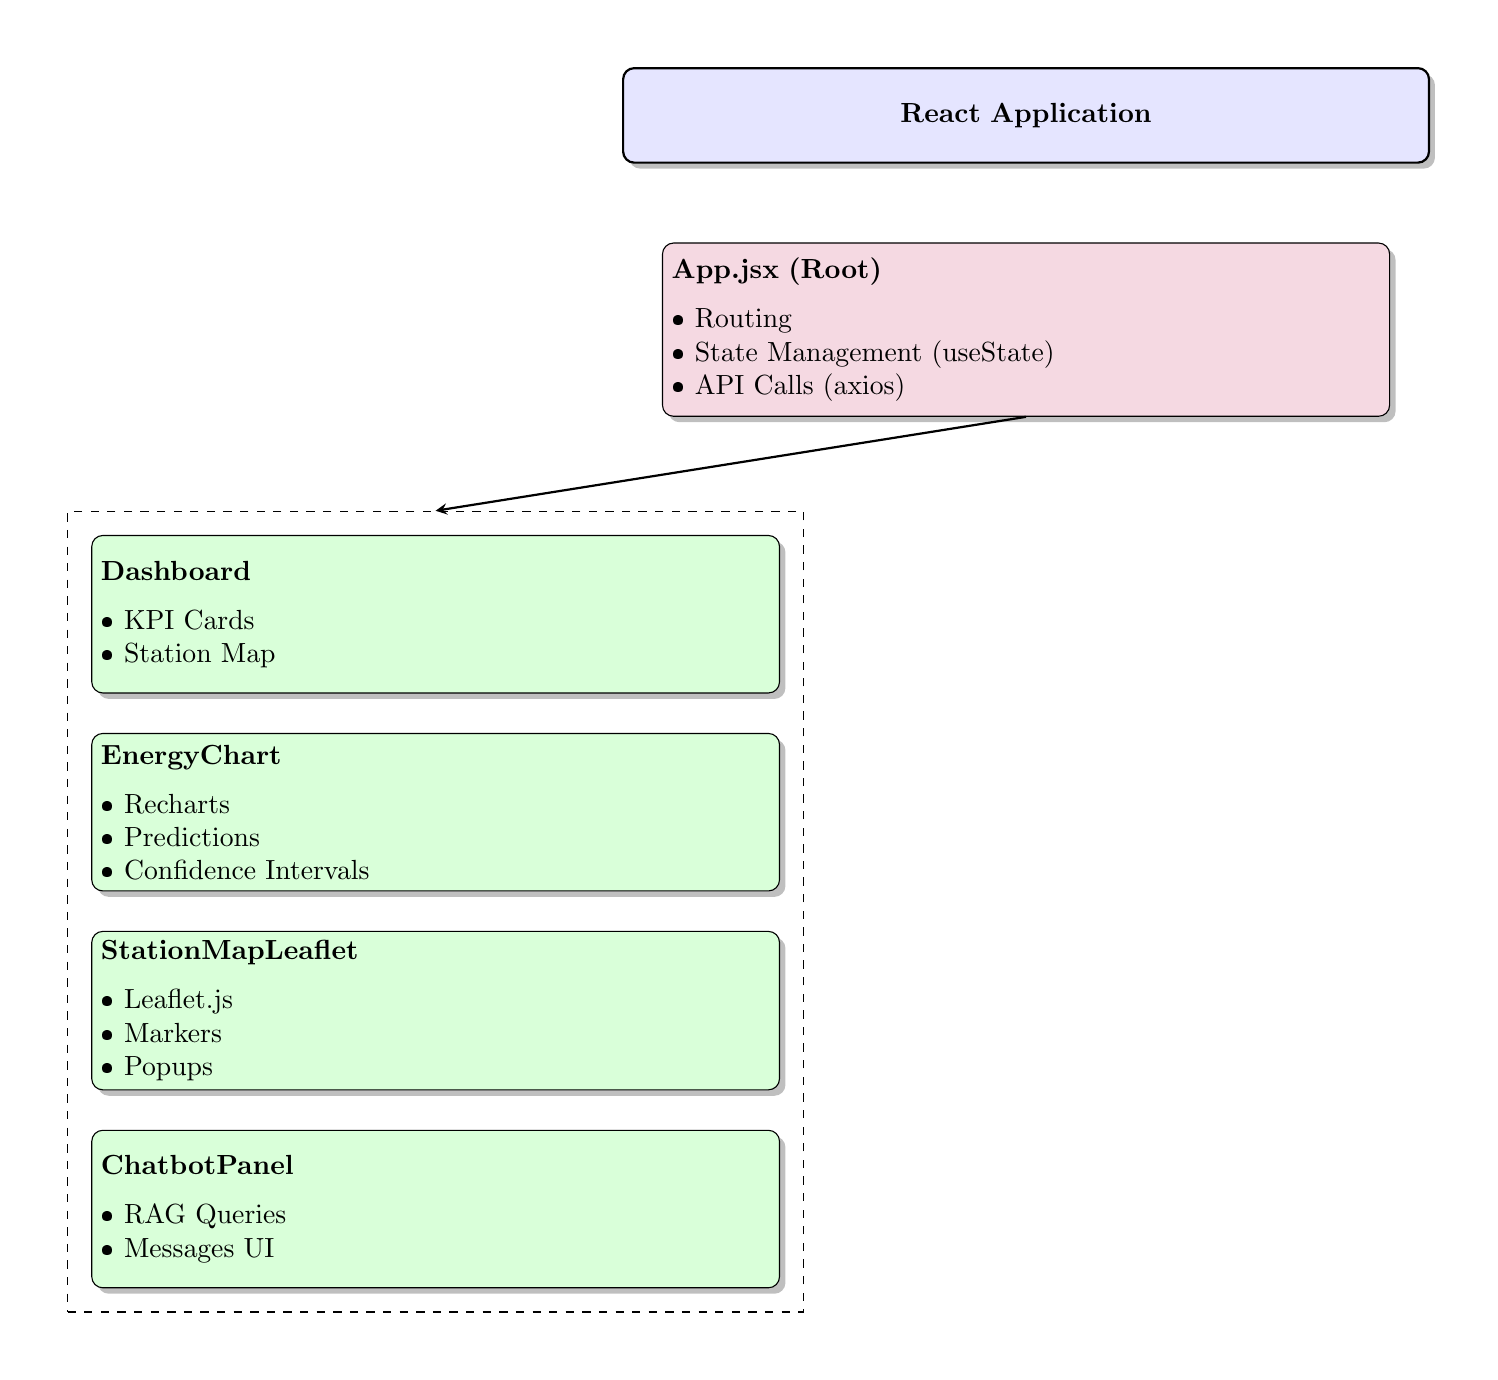
\begin{tikzpicture}[
    node distance=0.8cm,
    mainbox/.style={rectangle, draw, fill=blue!10, text width=10cm, minimum height=1.2cm, text centered, rounded corners, drop shadow, thick},
    rootbox/.style={rectangle, draw, fill=purple!15, text width=9cm, minimum height=2.2cm, align=left, rounded corners, drop shadow},
    compbox/.style={rectangle, draw, fill=green!15, text width=8.5cm, minimum height=2cm, align=left, rounded corners, drop shadow},
    arrow/.style={->, >=stealth, thick},
    label/.style={font=\small\bfseries}
]

% Main React App
\node[mainbox] (react) at (0,0) {
    \textbf{React Application}
};

% App.jsx Root
\node[rootbox, below=1cm of react] (app) {
    \textbf{App.jsx (Root)}\\[0.2cm]
    • Routing\\
    • State Management (useState)\\
    • API Calls (axios)
};

% Dashboard Component
\node[compbox, below left=1.5cm and -1.5cm of app] (dashboard) {
    \textbf{Dashboard}\\[0.2cm]
    • KPI Cards\\
    • Station Map
};

% EnergyChart Component
\node[compbox, below=0.5cm of dashboard] (chart) {
    \textbf{EnergyChart}\\[0.2cm]
    • Recharts\\
    • Predictions\\
    • Confidence Intervals
};

% StationMapLeaflet Component
\node[compbox, below=0.5cm of chart] (map) {
    \textbf{StationMapLeaflet}\\[0.2cm]
    • Leaflet.js\\
    • Markers\\
    • Popups
};

% ChatbotPanel Component
\node[compbox, below=0.5cm of map] (chatbot) {
    \textbf{ChatbotPanel}\\[0.2cm]
    • RAG Queries\\
    • Messages UI
};

% Component Tree Box
\node[draw, dashed, fit=(dashboard) (chart) (map) (chatbot), inner sep=0.3cm, label={[label, above]north:Components Tree}] (tree) {};

% Arrows
\draw[arrow] (app.south) -- (tree.north);

% Position adjustment
\node[fit=(react) (app) (tree), inner sep=0.5cm] {};

\end{tikzpicture}
\end{document}
